\documentclass[11pt,]{article}
\usepackage[left=1in,top=1in,right=1in,bottom=1in]{geometry}
\newcommand*{\authorfont}{\fontfamily{phv}\selectfont}
\usepackage[]{mathpazo}


  \usepackage[T1]{fontenc}
  \usepackage[utf8]{inputenc}




\usepackage{abstract}
\renewcommand{\abstractname}{}    % clear the title
\renewcommand{\absnamepos}{empty} % originally center

\renewenvironment{abstract}
 {{%
    \setlength{\leftmargin}{0mm}
    \setlength{\rightmargin}{\leftmargin}%
  }%
  \relax}
 {\endlist}

\makeatletter
\def\@maketitle{%
  \newpage
%  \null
%  \vskip 2em%
%  \begin{center}%
  \let \footnote \thanks
    {\fontsize{18}{20}\selectfont\raggedright  \setlength{\parindent}{0pt} \@title \par}%
}
%\fi
\makeatother




\setcounter{secnumdepth}{0}

\usepackage{longtable,booktabs}

\usepackage{graphicx,grffile}
\makeatletter
\def\maxwidth{\ifdim\Gin@nat@width>\linewidth\linewidth\else\Gin@nat@width\fi}
\def\maxheight{\ifdim\Gin@nat@height>\textheight\textheight\else\Gin@nat@height\fi}
\makeatother
% Scale images if necessary, so that they will not overflow the page
% margins by default, and it is still possible to overwrite the defaults
% using explicit options in \includegraphics[width, height, ...]{}
\setkeys{Gin}{width=\maxwidth,height=\maxheight,keepaspectratio}


\title{Making Migration Sexy: Immigrants in Same-Sex Couples in the United States \thanks{We appreciate\ldots.}  }



\author{\Large Nathan I. Hoffmann\vspace{0.05in} \newline\normalsize\emph{Department of Sociology, University of California, Los Angeles}   \and \Large Kristopher Velasco\vspace{0.05in} \newline\normalsize\emph{Departmnet of Sociology, University of Texas at Austin}  }


\date{}

\usepackage{titlesec}

\titleformat*{\section}{\normalsize\bfseries}
\titleformat*{\subsection}{\normalsize\itshape}
\titleformat*{\subsubsection}{\normalsize\itshape}
\titleformat*{\paragraph}{\normalsize\itshape}
\titleformat*{\subparagraph}{\normalsize\itshape}





\newtheorem{hypothesis}{Hypothesis}
\usepackage{setspace}


% set default figure placement to htbp
\makeatletter
\def\fps@figure{htbp}
\makeatother

\usepackage{fancyhdr}
\pagestyle{fancy}
\setlength{\headheight}{13.6pt}
\rhead{\textit{Hoffmann and Velasco}}

% move the hyperref stuff down here, after header-includes, to allow for - \usepackage{hyperref}

\makeatletter
\@ifpackageloaded{hyperref}{}{%
\ifxetex
  \PassOptionsToPackage{hyphens}{url}\usepackage[setpagesize=false, % page size defined by xetex
              unicode=false, % unicode breaks when used with xetex
              xetex]{hyperref}
\else
  \PassOptionsToPackage{hyphens}{url}\usepackage[draft,unicode=true]{hyperref}
\fi
}

\@ifpackageloaded{color}{
    \PassOptionsToPackage{usenames,dvipsnames}{color}
}{%
    \usepackage[usenames,dvipsnames]{color}
}
\makeatother
\hypersetup{breaklinks=true,
            bookmarks=true,
            pdfauthor={Nathan I. Hoffmann (Department of Sociology, University of California, Los Angeles) and Kristopher Velasco (Departmnet of Sociology, University of Texas at Austin)},
             pdfkeywords = {immigration, same-sex couples, LGBTQ policy},  
            pdftitle={Making Migration Sexy: Immigrants in Same-Sex Couples in the United States},
            colorlinks=true,
            citecolor=blue,
            urlcolor=blue,
            linkcolor=blue,
            pdfborder={0 0 0}}
\urlstyle{same}  % don't use monospace font for urls

% Add an option for endnotes. -----


% add tightlist ----------
\providecommand{\tightlist}{%
\setlength{\itemsep}{0pt}\setlength{\parskip}{0pt}}

% add some other packages ----------

% \usepackage{multicol}
% This should regulate where figures float
% See: https://tex.stackexchange.com/questions/2275/keeping-tables-figures-close-to-where-they-are-mentioned
\usepackage[section]{placeins}


\begin{document}
	
% \pagenumbering{arabic}% resets `page` counter to 1 
%
% \maketitle

{% \usefont{T1}{pnc}{m}{n}
\setlength{\parindent}{0pt}
\thispagestyle{plain}
{\fontsize{18}{20}\selectfont\raggedright 
\maketitle  % title \par  

}

{
   \vskip 13.5pt\relax \normalsize\fontsize{11}{12} 
\textbf{\authorfont Nathan I. Hoffmann} \hskip 15pt \emph{\small Department of Sociology, University of California, Los Angeles}   \par \textbf{\authorfont Kristopher Velasco} \hskip 15pt \emph{\small Departmnet of Sociology, University of Texas at Austin}   

}

}








\begin{abstract}

    \hbox{\vrule height .2pt width 39.14pc}

    \vskip 8.5pt % \small 

\noindent Galvanized by greater social acceptance and new rights, numbers of same-sex couples in the United States are increasing, yet few demographers have studied immigrants in same-sex couples. Using the American Community Survey from 2008 to 2018, this study compares same-sex couples including at least one immigrant to corresponding opposite-sex couples in order to characterize and assess the scale of sexual migration to the U.S. Moreover, we evaluate how the policy environment related to same-sex couples shapes migratory patterns. We find that same-sex couples generally have higher incomes and occupational prestige and are somewhat more educated. Moreover these couples are influenced by LGBT policies, both in their origin country and their U.S. state destination, and are less influenced by previous migration of conationals. Our findings put into question predominant models of migration that emphasize economic and and network effects, suggesting the importance of considering political and lifestyle motivations.


\vskip 8.5pt \noindent \emph{Keywords}: immigration, same-sex couples, LGBTQ policy \par

    \hbox{\vrule height .2pt width 39.14pc}



\end{abstract}


\vskip -8.5pt


 % removetitleabstract

\noindent  

\hypertarget{data}{%
\section{Data}\label{data}}

\hypertarget{methods}{%
\section{Methods}\label{methods}}

\hypertarget{results}{%
\section{Results}\label{results}}

\hypertarget{descriptive-statistics}{%
\subsection{Descriptive statistics}\label{descriptive-statistics}}

\begin{table}

\caption{\label{tab:state-table}States ranked by average estimated number of couples containing one or two immigrants}
\centering
\begin{tabular}[t]{lllll}
\toprule
Different-sex rank & State  &   & Same-sex rank & State\\
\midrule
1 & California &  & 1 & California\\
2 & Texas &  & 2 & New York\\
3 & New York &  & 3 & Florida\\
4 & Florida &  & 4 & Texas\\
5 & New Jersey &  & 5 & New Jersey\\
6 & Illinois &  & 6 & Illinois\\
7 & Washington &  & 7 & Massachusetts\\
8 & Virginia &  & 8 & Washington\\
9 & Massachusetts &  & 9 & Virginia\\
10 & Georgia &  & 10 & Pennsylvania\\
\bottomrule
\end{tabular}
\end{table}

\begin{table}

\caption{\label{tab:table-prop}States ranked by proportion immigrant couples with same-sex partners}
\centering
\begin{tabular}[t]{lll}
\toprule
Rank & State or district & Proportion same-sex\\
\midrule
1 & District of Columbia & 6.19 \%\\
2 & Vermont & 2.09 \%\\
3 & Maine & 1.63 \%\\
4 & Montana & 1.47 \%\\
5 & Missouri & 1.18 \%\\
6 & Massachusetts & 1.12 \%\\
7 & New York & 1.1 0\%\\
8 & Florida & 1.01 \%\\
9 & Mississippi & 1 .00\%\\
10 & Minnesota & 0.96 \%\\
\bottomrule
\end{tabular}
\end{table}

\begin{table}

\caption{\label{tab:country-tab}Sending countries ranked by proportion U.S. immigrants in same-sex couples}
\centering
\begin{tabular}[t]{lll}
\toprule
Rank & Country of origin & Proportion same-sex\\
\midrule
1 & Australia & 2.53 \%\\
2 & Mongolia & 2.37 \%\\
3 & Belgium & 2.25 \%\\
4 & New Zealand & 2.12 \%\\
5 & Singapore & 2.11 \%\\
6 & Netherlands & 2.08 \%\\
7 & France & 2.05 \%\\
8 & Malaysia & 2.05 \%\\
9 & Zimbabwe & 2.01 \%\\
10 & Spain & 1.98 \%\\
\bottomrule
\end{tabular}
\end{table}

\begin{figure}
\centering
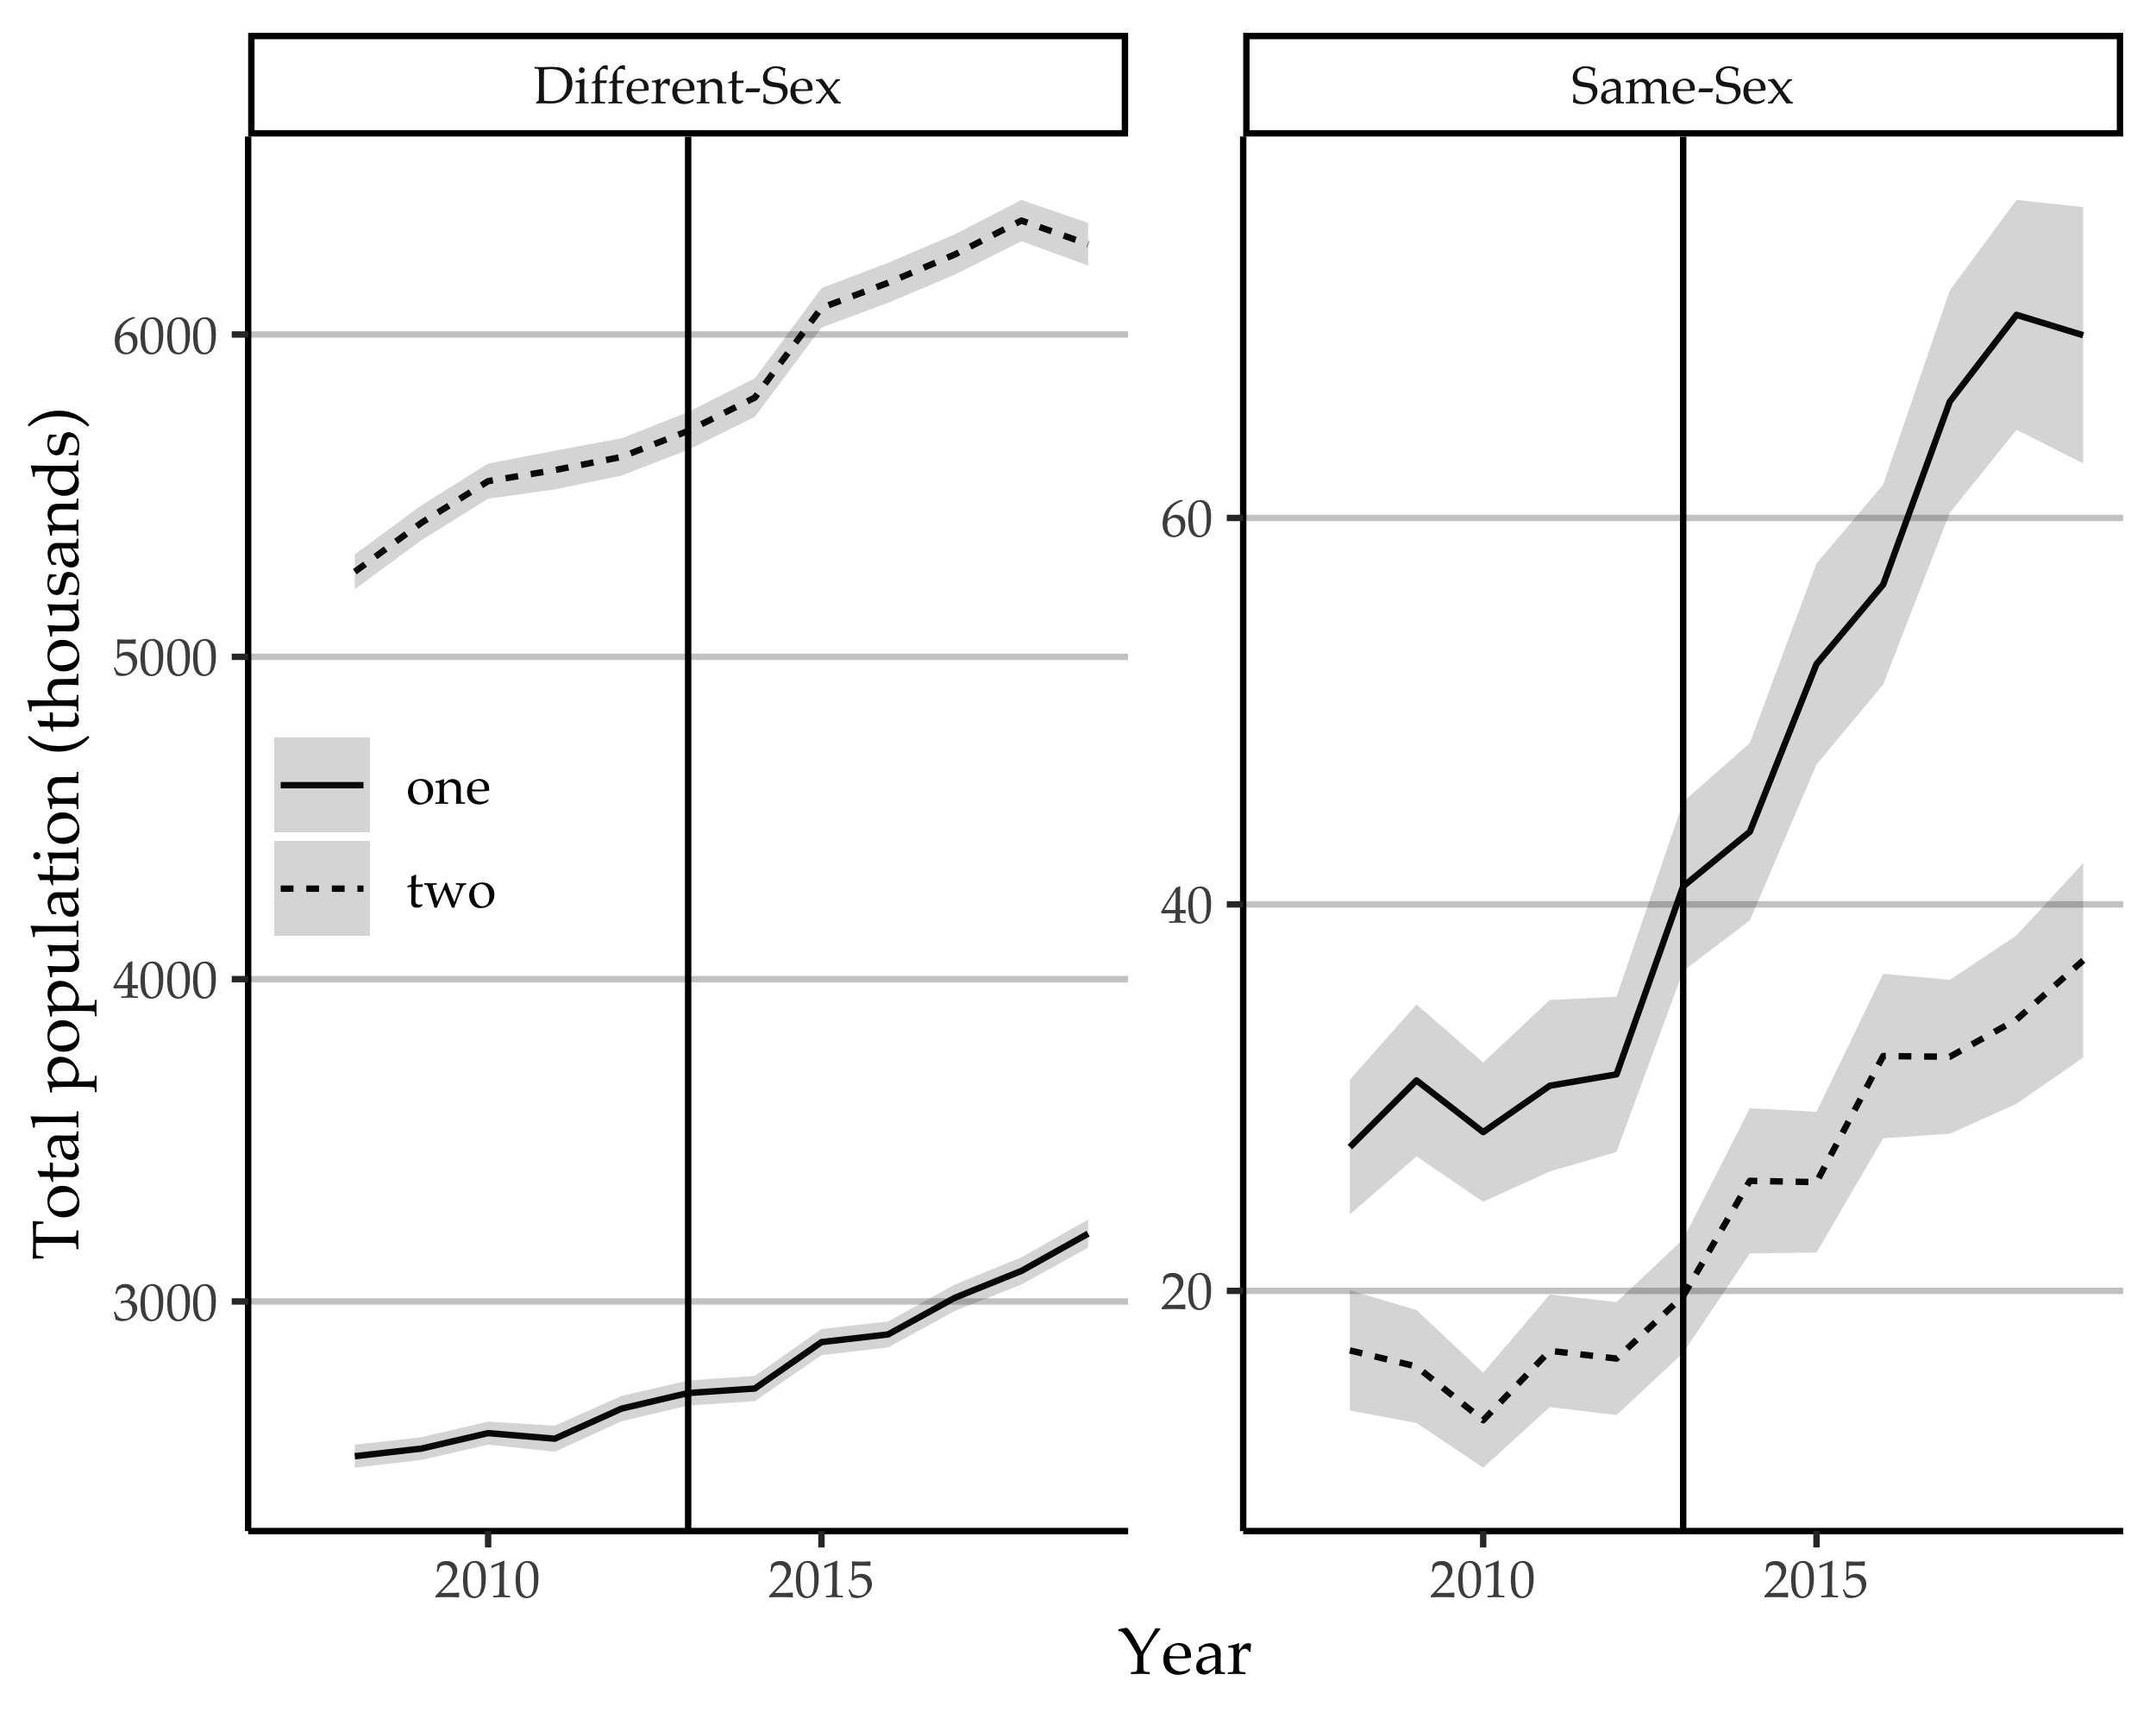
\includegraphics{ssimm_draft_methods_results_files/figure-latex/total-pop-1.pdf}
\caption{\label{fig:total-pop}Estimated totals of different- and same-sex couples containing one or two immigrants, 2008-2019}
\end{figure}

\hypertarget{models}{%
\subsection{Models}\label{models}}

\begin{table}[!htbp] \centering 
  \caption{100*Proportion same-sex in a country-year of immigration} 
  \label{tab:country-props} 
\begin{tabular}{@{\extracolsep{5pt}}lcccc} 
\\[-1.8ex]\hline 
\hline \\[-1.8ex] 
 & \multicolumn{4}{c}{\textit{Dependent variable:}} \\ 
\cline{2-5} 
\\[-1.8ex] & \multicolumn{4}{c}{prop\_same\_sex} \\ 
\\[-1.8ex] & (1) & (2) & (3) & (4)\\ 
\hline \\[-1.8ex] 
 origin\_score & 0.079$^{***}$ &  & 0.066$^{***}$ & 0.037$^{+}$ \\ 
  & (0.007) &  & (0.010) & (0.019) \\ 
  & & & & \\ 
 distw &  & 0.00002$^{*}$ & 0.00003$^{**}$ & 0.002$^{*}$ \\ 
  &  & (0.00001) & (0.00001) & (0.001) \\ 
  & & & & \\ 
 contig &  & 0.110 & $-$0.037 & 2.500$^{+}$ \\ 
  &  & (0.200) & (0.200) & (1.500) \\ 
  & & & & \\ 
 comlang\_off &  & $-$0.012 & 0.003 & $-$17.000$^{*}$ \\ 
  &  & (0.081) & (0.081) & (7.900) \\ 
  & & & & \\ 
 comlang\_ethno &  & $-$0.051 & 0.010 & 8.500$^{*}$ \\ 
  &  & (0.069) & (0.069) & (3.800) \\ 
  & & & & \\ 
 colony &  & 0.300$^{*}$ & 0.120 & 12.000$^{*}$ \\ 
  &  & (0.140) & (0.140) & (5.700) \\ 
  & & & & \\ 
 wage\_dif &  & 0.00001 & $-$0.00001 & 0.00001 \\ 
  &  & (0.00001) & (0.00001) & (0.00001) \\ 
  & & & & \\ 
 unemp\_dif &  & $-$0.002 & $-$0.002 & 0.005 \\ 
  &  & (0.004) & (0.004) & (0.009) \\ 
  & & & & \\ 
 polity5 &  & 0.036$^{***}$ & 0.023$^{***}$ & 0.0004 \\ 
  &  & (0.004) & (0.005) & (0.010) \\ 
  & & & & \\ 
\hline \\[-1.8ex] 
Country-clustered SEs? & yes & yes & yes & yes \\ 
Country FEs? & no & no & no & yes \\ 
Observations & 3,811 & 2,995 & 2,995 & 2,995 \\ 
R$^{2}$ & 0.031 & 0.028 & 0.041 & 0.120 \\ 
\hline 
\hline \\[-1.8ex] 
\textit{Note:}  & \multicolumn{4}{r}{$^{*}$p$<$0.1; $^{**}$p$<$0.05; $^{***}$p$<$0.01} \\ 
 & \multicolumn{4}{r}{+p<0.1; *p<0.05; **p<0.01; ***p<0.001} \\ 
\end{tabular} 
\end{table}

\begin{table}[!htbp] \centering 
  \caption{100*Proportion same-sex in a country-state-year} 
  \label{tab:state-props} 
\begin{tabular}{@{\extracolsep{5pt}}lccc} 
\\[-1.8ex]\hline 
\hline \\[-1.8ex] 
 & \multicolumn{3}{c}{\textit{Dependent variable:}} \\ 
\cline{2-4} 
\\[-1.8ex] & \multicolumn{3}{c}{same\_prop} \\ 
\\[-1.8ex] & (1) & (2) & (3)\\ 
\hline \\[-1.8ex] 
 state\_unemploy &  & $-$0.033$^{+}$ & $-$0.001 \\ 
  &  & (0.017) & (0.023) \\ 
  & & & \\ 
 state\_income &  & 0.00001 & $-$0.00003 \\ 
  &  & (0.00001) & (0.00002) \\ 
  & & & \\ 
 origin\_score & 0.053$^{***}$ & 0.050$^{***}$ & 0.110$^{**}$ \\ 
  & (0.011) & (0.011) & (0.040) \\ 
  & & & \\ 
 distw &  &  & 0.004$^{***}$ \\ 
  &  &  & (0.001) \\ 
  & & & \\ 
 contig &  &  & 5.900$^{***}$ \\ 
  &  &  & (1.600) \\ 
  & & & \\ 
 comlang\_off &  &  & $-$35.000$^{***}$ \\ 
  &  &  & (8.600) \\ 
  & & & \\ 
 comlang\_ethno &  &  & 18.000$^{***}$ \\ 
  &  &  & (4.100) \\ 
  & & & \\ 
 colony &  &  & 26.000$^{***}$ \\ 
  &  &  & (6.200) \\ 
  & & & \\ 
 wage\_dif &  &  & 0.0001$^{**}$ \\ 
  &  &  & (0.0001) \\ 
  & & & \\ 
 unemp\_dif &  &  & $-$0.022$^{+}$ \\ 
  &  &  & (0.012) \\ 
  & & & \\ 
 polity5 &  &  & $-$0.001 \\ 
  &  &  & (0.012) \\ 
  & & & \\ 
 state\_policy & 0.033$^{+}$ & 0.008 & 0.041 \\ 
  & (0.017) & (0.034) & (0.036) \\ 
  & & & \\ 
\hline \\[-1.8ex] 
State-clustered SEs? & yes & yes & yes \\ 
State FEs? & no & yes & yes \\ 
Country FEs? & no & no & yes \\ 
Observations & 44,431 & 44,076 & 39,147 \\ 
R$^{2}$ & 0.001 & 0.003 & 0.010 \\ 
\hline 
\hline \\[-1.8ex] 
\textit{Note:}  & \multicolumn{3}{r}{+p<0.1; *p<0.05; **p<0.01; ***p<0.001} \\ 
\end{tabular} 
\end{table}

\begin{table}[!htbp] \centering 
  \caption{Individual ordered logit analysis of three-category state policy score} 
  \label{tab:ord} 
\begin{tabular}{@{\extracolsep{5pt}}lccc} 
\\[-1.8ex]\hline 
\hline \\[-1.8ex] 
 & \multicolumn{3}{c}{\textit{Dependent variable:}} \\ 
\cline{2-4} 
\\[-1.8ex] & \multicolumn{3}{c}{state\_policy\_binned} \\ 
\\[-1.8ex] & (1) & (2) & (3)\\ 
\hline \\[-1.8ex] 
 same\_sex & 0.160$^{***}$ & 0.100$^{***}$ & 20.000$^{***}$ \\ 
  & (0.020) & (0.027) & (0.0003) \\ 
  origin\_score &  & $-$0.051$^{***}$ & $-$0.022$^{***}$ \\ 
  &  & (0.003) & (0.003) \\ 
  sexMale &  &  & $-$0.059$^{***}$ \\ 
  &  &  & (0.013) \\ 
  age &  &  & 0.001$^{+}$ \\ 
  &  &  & (0.001) \\ 
  educcollege &  &  & 0.070$^{***}$ \\ 
  &  &  & (0.010) \\ 
  educHS &  &  & $-$0.036$^{***}$ \\ 
  &  &  & (0.011) \\ 
  educsome col &  &  & $-$0.023$^{*}$ \\ 
  &  &  & (0.011) \\ 
  nchild &  &  & 0.045$^{***}$ \\ 
  &  &  & (0.006) \\ 
  log\_income &  &  & 0.070$^{***}$ \\ 
  &  &  & (0.002) \\ 
  no\_income &  &  & 0.610$^{***}$ \\ 
  &  &  & (0.002) \\ 
  yrimmig &  &  & $-$0.020$^{***}$ \\ 
  &  &  & (0.00002) \\ 
  same\_sexTRUE:origin\_score &  & 0.038$^{***}$ & 0.052$^{***}$ \\ 
  &  & (0.008) & (0.009) \\ 
  same\_sexTRUE:sexMale &  &  & 0.041$^{***}$ \\ 
  &  &  & (0.002) \\ 
  same\_sexTRUE:age &  &  & $-$0.005$^{***}$ \\ 
  &  &  & (0.002) \\ 
  same\_sexTRUE:educcollege &  &  & 0.120$^{***}$ \\ 
  &  &  & (0.003) \\ 
  same\_sexTRUE:educHS &  &  & 0.005$^{**}$ \\ 
  &  &  & (0.002) \\ 
  same\_sexTRUE:educsome col &  &  & 0.064$^{***}$ \\ 
  &  &  & (0.001) \\ 
  same\_sexTRUE:nchild &  &  & $-$0.017 \\ 
  &  &  & (0.021) \\ 
  same\_sexTRUE:log\_income &  &  & 0.029$^{***}$ \\ 
  &  &  & (0.006) \\ 
  same\_sexTRUE:no\_income &  &  & 0.290$^{***}$ \\ 
  &  &  & (0.001) \\ 
  same\_sexTRUE:yrimmig &  &  & $-$0.010$^{***}$ \\ 
  &  &  & (0.0001) \\ 
 \hline \\[-1.8ex] 
Country-clustered SEs? & yes & yes & yes \\ 
Survey year FEs? & yes & yes & yes \\ 
Observations & 111,880 & 107,168 & 107,168 \\ 
\hline 
\hline \\[-1.8ex] 
\textit{Note:}  & \multicolumn{3}{r}{+p<0.1; *p<0.05; **p<0.01; ***p<0.001} \\ 
\end{tabular} 
\end{table}

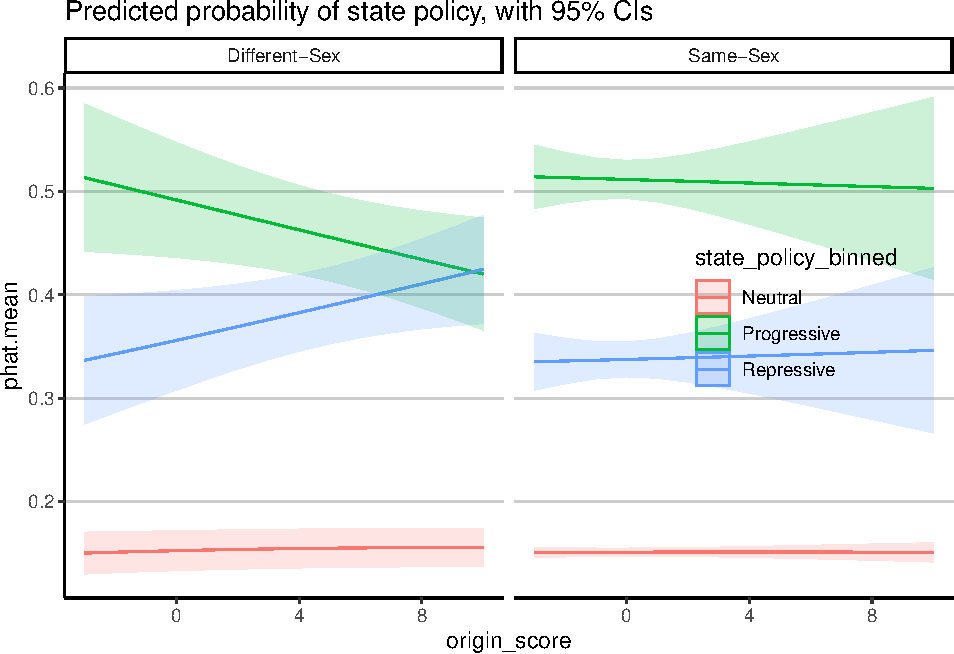
\includegraphics{ssimm_draft_methods_results_files/figure-latex/sim-1.pdf}

\hypertarget{references}{%
\section{References}\label{references}}

\setlength{\parindent}{-0.2in}
\setlength{\leftskip}{0.2in}
\setlength{\parskip}{8pt}

\noindent

\newpage
\singlespacing 
\end{document}
